\documentclass[a4paper,11pt]{article}
\usepackage[style=mla,style=authoryear,backend=biber]{biblatex}
\renewcommand*{\nameyeardelim}{\addcomma\space}  % add comma between author and year
\usepackage{soul}
\usepackage{hyperref}
\usepackage[colorinlistoftodos]{todonotes}
\usepackage{calc}  % importent in order to import inkspace images
\usepackage[labelfont=bf]{caption}  % set caption label to bold
\usepackage{enumitem}  % to interrupt enumerations and resume
\usepackage{amsmath}
\usepackage{tabularx}  % alternative tabular package for the surveys
\newcolumntype{Y}{>{\centering\arraybackslash}X}  % for centered columns
\usepackage[toc,page]{appendix}
\pdfobjcompresslevel=0  % fixing acrobat error 131

\addbibresource{bibliography.bib}

\graphicspath{ {images/}{graphics/}{plots/} }

\newcommand{\definition}[1]{\emph{#1}}
\newcommand{\noriinline}[1]{\todo[author=Nori,inline,color=green]{#1}}
\newcommand{\nori}[1]{\todo[author=Nori,color=green]{#1}}
\newcommand{\myunderline}{\rule{2in}{.5pt}}

\title{An Audio-Only Augmented Reality System for\\Social Interaction}
\author{Tom Gurion}

\begin{document}
\maketitle

% \listoftodos
\tableofcontents

\section{Introduction}

Over the past sixty years the development of new technologies has fundamentally transformed music creation and consumption (\cite{hargreaves99}).
One outcome has been the emergence of interactive music systems (IMS) which facilitate new modes of music creation by blurring the traditional distinction between instrument design, composition and performance (\cite{drummond09}).
In recent years there have been many attempts to provide IMS not only to professional musicians, but also directly to the average user (\cite{stimulant13}).

This research aligns with this trend by exploring new possibilities for joint interactive music consumption by a group of users.
I developed an audio-only augmented reality system that facilitates social interactions.
The system is mainly motivated by silent disco, flash mobs and augmented reality, and aims to create an interactive space in which users can move, interact, and thus affect the music they and their companions hear in their headphones.
Throughout this study the system is presented as a silent disco use case.
Nevertheless, the system is characterized by a modular architecture which can be extended to other uses and further exploration of the system's interactive behavior.

I hypothesised that the system can enhance social interactions between its users.
In addition, two additional hypotheses were formulated.
These were (a) that participating in a party using the system would strengthen the social relationships between participants even beyond the scope of the party and (b) that the system alters in-group cohesion and the individual's openness to out-group social interactions.

I assessed the social effects of system use in two experiments in the context of silent disco party.
The results of the first experiment show that the system indeed facilitates social interactions between the users of the system.
The second experiment fine-tunes the insights of the first experiment by presenting a complex set of movement and gathering patterns.
These results are integrated to form a novel model for enhanced social interaction, thus revealing the potential of using audio-only augmented reality in future interactive experiences.

\section{Literature review}

The current work is based on interdisciplinary research.
The following sections review these domains and emphasize the projects, technologies, and research that serve as the foundation for both the development and evaluation of my system.

In sections \ref{literature:ims} and \ref{literature:non_pro_ims} I present the history of IMS and recent trends related to my study.
Sections \ref{literature:social_tech} and \ref{literature:ar} discuss the rationale for the system development.
Some specific technological background on system development dealing with the indoor positioning capabilities of mobile devices, is presented in section \ref{literature:ips}.
Finally, section \ref{literature:social_effects} briefly reviews the social effects of music and discusses ways to evaluate my system.

\subsection{The origins of interactive music systems} \label{literature:ims}

According to the Oxford English Dictionary, to \emph{interact} is to ``act in such a way as to have an effect on each other''.
In the field of IMS, actions and effects can draw on a broad spectrum of novel techniques ranging from interactive sound installations to collaborations with robotic performers (\cite{drummond09}).

Traditionally, IMS merges developments from several different sources to facilitate new modes of music creation.
Music-oriented programming languages such as the MUSIC-N series and Max/MSP (\cite{mathews69}; \cite[p. 16]{winkler01}), standardization of technologies such as MIDI (\cite{web:quinn}), the role of the personal computer in music production (\cite{leider:04}), and the recent emergence of the ``makers culture'' (\cite{kuznetsov2010rise}) are only a few of these threads.
I briefly review the key features of these trends.

Ever since the early forays into the field of IMS in the 1960s, different researchers and composers have created systems designed to interact with performers in a live situation.
Perhaps the first example of this kind of interactive system is Gordon Mumma's Hornpipe, a specially designed electronic system that alters the audio input from the performer by creating an interactive loop between the player and the sound emitted by the electronics circuit (\cite[p. 12]{winkler01}).

In the 1970s musicians and researchers started to use newly developed programming languages designed specifically for musical applications such as GROOVE or the MUSIC-N series (\cite{mathews70}; \cite{mathews69}).
As pioneering technologies for digital sound synthesis, these programming languages gained wide acceptance in the music research community and became the seedbed for the new genre and field of research of computer music.

Charles Dodge's ``Earth's Magnetic Fields'' is one of the earliest computer music compositions, and is a good example of its new and unique possibilities.
In this piece, magnetic field readings were collected over the course of a year.
Later, Dodge mapped the readings to a four octave span, applying interpolation between readings that manipulated the tempo and dynamics of the music (\cite{scriptsgrooves14}).
This approach in which the composer sets down a set of rules and applies them to input data to generate musical materials automatically was unprecedented, and contrasted with the main technique that involved composing electronic music by cutting and pasting magnetic tapes manually.

In 1983, a group of musical instruments manufacturers agreed on a universal standard for digitally sending and receiving musical information known as the MIDI protocol (\cite{web:quinn}).
This standardization, combined with the emergence of personal computers, was the impetus for the creation of modern programing languages for musical applications.
Unlike early programming languages such as GROOVE or the MUSIC-N series, most personal-computer-based languages still exist today and have continued to evolve.
A prominent example is Max/MSP, which was first developed by Miller Puckette in 1986 (\cite[p. 16]{winkler01})\footnote{Max 6, the recent version of Max/MSP: \href{http://cycling74.com/products/max/}{cycling74.com/products/max/}.}.
Moreover, new music-oriented programing languages are being developed today, and have features including ``on-the-fly'' programming (the ability to change the features of the program during run-time)\footnote{ChucK: \href{http://chuck.cs.princeton.edu/}{chuck.cs.princeton.edu/}.}, web capabilities\footnote{The Web audio API: \href{http://www.w3.org/TR/webaudio/}{www.w3.org/TR/webaudio/}.} and modular environment for live performance (that also make use of a mobile multi-touch interface)\footnote{Usine Hollyhock: \href{http://www.sensomusic.org/}{www.sensomusic.org/}.}.

Similar technological shifts have also prompted the use of personal computers as a central component in the modern recording studio, thereby establishing the role of PCs as a commonplace alternative to analog recording equipment (\cite{leider:04}).
With the arrival of Virtual Studio Technology (VST) as the standard for digital signal processing plug-ins, computers became an even more essential tool for music production.
These developments paralleled the emergence of live performance-oriented software as Ableton Live\footnote{Ableton Live: \href{http://www.ableton.com/en/live/}{www.ableton.com/live/}.} and software based DJ setups at the late 1990s.

Another key event in the history of IMS was the appearance of the Arduino platform in 2006.
Arduino is an easy-to-use hardware and software package intended for interactive objects or environment creation\footnote{Arduino: \href{http://arduino.cc/}{arduino.cc/}.}.
By translating physical properties into sound, the Arduino platform paved the way for musicians to use more than just audio and MIDI to communicate with music creation software in interactive environments.

More generally, Arduino can be seen as an important part of the new ``makers'' movements, a technology-based extension of the ``do it yourself'' culture.
``Makers'' are usually highly trained programmers who use open source software and basic electronics to create mashes of electronics and real world objects.
By creating what used to be purchased, and usually open-sourcing it (sharing this knowledge with the community), the makers have become a major driving force in the development of IMS (\cite{web:kirn12}).

Today, the makers movement can be considered the unofficial host for several IMS projects by independent makers who present their works in different fairs around the world.
The vast number of dedicated web pages for musical projects in makers' websites illustrates the strong link between music and the makers community\footnote{Examples: \href{http://blog.arduino.cc/category/music/}{blog.arduino.cc/category/music/}; \href{http://makerfaire.com/category/music/}{makerfaire.com/category/music/}}.

\subsection{Interactive music systems for non-professional musicians} \label{literature:non_pro_ims}

Today, non-professional musicians have access to IMS in a variety of scenarios, including interactive video clips, mobile and album applications, interactive sound installations, and social DJing.
These typical examples are only a small portion of the novel ways in which non-professionals can now be involved in interactive music creation and use of audiovisual content as well as musically enhanced social interactions.

% interactive video clips: Interlude, Chris Milk and Aaron Koblin
Interactive video clips allow users to interact with videos in ways that traditionally were limited to the director of the video clip.
As a relatively new phenomenon, interactive video clips have become increasingly visible in popular culture.
A good example are works by Chris Milk and Aaron Koblin, in which the video clip runs on a dedicated webpage and responds to the users by tracking their mouse, keyboard strokes, or other inputs\footnote{Milk and Koblin's projects: \href{http://www.thewildernessdowntown.com/}{www.thewildernessdowntown.com/}; \href{http://www.ro.me/}{www.ro.me/}.}.
In Milk's project ``ROME - 3 dreams of black'', the user is presented with three dimensional world in which the video clip takes place.
During the clip the user can choose a direction to focus on using the mouse, which also affects the visual image around the pointed area.
At the end, the user is invited to create new three dimensional objects, using an editor in the browser, which is then added to the virtual world of the clip for future visitors.

A similar approach can also be found in interactive video clips created by the startup Interlude\footnote{Interlude: \href{http://interlude.fm/}{interlude.fm/}.}, Beck's recent project ``Hello again''\footnote{Beck's ``Hello again'': \href{http://www.hello-again.com/beck360/}{www.hello-again.com/beck360/}.} and others.
In contrast to ``ROME'', where the interaction with the video clip only manipulates the visual output, in some of the other projects mentioned above the manipulation affects both the auditory and visual domains.

% mobile applications: Smule and RjDj
Mobile phones, which until recently were merely a communication tool, are rapidly incrementing computational capability and comprehensive features each year.
These improvements have changed the way users interact with mobile devices and are contributing to the development of new IMS for non-professional musicians.
It comes as no surprise that the number of musical mobile applications that integrate interactive components is constantly on the rise.
For example, AutoRap turns speech into rap by slicing the syllables and mapping them according to different beat styles\footnote{Smule's AutoRap: \href{https://play.google.com/store/apps/details?id=com.smule.autorap}{https://play.google.com/store/apps/details?id=com.smule.autorap}.}.
Other examples are applications by Brian Eno and Peter Chilvers, which enable users to compose music simply by using visual elements on the device screen\footnote{Generative music: \href{http://www.generativemusic.com/}{www.generativemusic.com/}.}.
Another interesting mobile project is RjDj, which uses phone sensors to create ambient sonification based on the users' interactions with their daily environment (\cite{web:rjdj})\label{rjdj}.

% album applications
Album applications are another new trend where artists are releasing their music as interactive applications for mobile devices.
A good example of this trend is the Icelandic musician Bj\"{o}rk's latest album, ``Biophilia'', which accompanies each of its 10 songs with a separate interactive experience (\cite{stimulant13}).
In Biophilia, users are encouraged to interact with the musical material visually to alter the compositional blocks (e.g.\ phrases and instruments) at will.
In addition to this interactive mode, termed the ``play'' mode in the application jargon, there are other interesting modes in this album application that the user can choose from.
Score mode, for example, resembles a type of karaoke, and the animation mode, presents an animated video-clip of the song.

% interactive sound installations: objects with sound, project ADA
Another concept that influenced this thesis is sound installations located in three-dimensional space that communicate with the audience through sound.
In some interactive sound installations the main interaction is between the viewer and the installation itself (\cite{web:visnjic}; \cite{web:cardiff01}) whereas in others, the main objective is to facilitate social interaction between participants (\cite{eng03}; \cite{web:kirn12}; \cite{web:murray-browne13}).

% social DJing: DistributedDJ, the BLOB and playmysong
A number of recent projects have suggested distributing the DJ role among participants so they can choose the music by themselves, thereby generating a playlist dynamically according to their musical tastes (\cite{web:shaw}), or distributing the DJ controllers among several participants, thus allowing each to control a different component of the music (\cite{web:shapira}).
Most of these projects are implemented as mobile or web applications, and some even integrate social elements\footnote{Playmysong: \href{http://www.playmysong.com/}{www.playmysong.com/}; The BLOB \href{http://vimeo.com/7338120}{vimeo.com/7338120}.}.

\subsection{Technology dependent social networking} \label{literature:social_tech}

Silent disco and flash mobs are two contemporary social trends that constitute the conceptual roots of this project.
They are both exemplifications of modern types of social behavior that tap the rapid growth of social media and newly available technologies.
The assumptions and models in this thesis start from the context of a silent disco party, and are inspired by flash mobs with respect to their use of new technologies to facilitate creative and artistic social behaviors.

Silent disco is a form of partying where the music is heard through headphones instead of loudspeakers.
This new phenomenon changes the nature of an ordinary party.
One way is to have two DJs spin completely different sets side by side at the same party, allowing each participant, who has two-channel wireless headphones, to decide which DJ to listen to\footnote{Headphone Disco: \href{http://headphonedisco.com/show.php}{headphonedisco.com/show.php}.}.
Another alternative is to have no DJ at all, and let each participant choose what music to hear individually, through his or her mobile device and headphones.

Flash mobs are public gatherings of people organized through social media to perform a short act together.
The unique aspects of this relatively new phenomenon have led researchers to suggest that the emergence of flash mobs is a significant event in the history of mobile communication (\cite{nicholson05}) and that it inherently reflects an artistic intent (\cite{brejzek10}).

\subsection{Augmented reality} \label{literature:ar}

According to Azuma ``augmented reality (AR) enhances a user's perception of and interaction with the real world''.
This concept usually relates to the visual modality: ``AR systems integrate 3-D virtual objects into a 3-D real environment in real time'' (\cite{azuma97}).

Today's augmented reality systems include wearable devices that can superimpose a computer-generated image on the users' view of the real world (e.g\ Google glass\footnote{Google glass: \href{http://www.google.com/glass/start/}{www.google.com/glass/start/}.} and Meta\footnote{Meta: \href{https://www.spaceglasses.com/}{www.spaceglasses.com/}.}) and applications for mobile devices for several purposes, ranging from driving aids (iOnRoad\footnote{iOnRoad: \href{http://www.ionroad.com/}{www.ionroad.com/}.}) to marketing (\cite{ikea}).

My work extends the definition of an AR system from the visual to the auditory modality.
Although it is based on a similar rationale, it is applied differently.
In this study I use AR as a way to enhance the user's experience through external technological devices that integrate into his / her physical environment.
Hence, the ``enhancers'' are the musical materials the users hear through their headphones, whereas ``augmented experience'' refers to enhanced social interactions.
More generally, this approach to AR may be applied to more comprehensive experiences of virtual environments.

\subsection{Indoor positioning systems} \label{literature:ips}

The system I propose requires the ability to locate the positioning of the users within an indoor environment.
As discussed below this is a non-trivial requirement.

Today, outdoor positioning systems are an integral part of the mobile environment as delivered mainly by the General Positioning System (GPS) which is available in any modern mobile device.
On the other hand, indoor positioning systems (IPS) have not yet been standardized, and therefore are still unavailable to the average user (\cite{web:turetsky}).

Recent research has found that WiFi is the preferred IPS technology for mobile devices.
WiFi-based systems can also enhance accuracy by applying inertial navigation using the device's additional sensors, such as its accelerometer, gyroscope, and compass (\cite{web:harrop}).
Note however that those solutions depend on the deployment of a WiFi infrastructure in every indoor environment where positioning information in desired.

A relatively new technology in the world of IPS is Bluetooth low energy (LE)\footnote{Bluetooth LE: \href{http://www.bluetooth.com/Pages/low-energy-tech-info.aspx}{www.bluetooth.com/Pages/low-energy-tech-info.aspx}}.
Using this technology, supported devices can roughly approximate the distance of nearby mobile tokens within a radius of 10 meters or so.
One indication of the success of Bluetooth LE is Apple's integration with their iBeacon IPS (\cite{web:danova});
Estimote\footnote{Estimote: \href{http://estimote.com/}{estimote.com/}.}, one of the largest iBeacon manufacturers, recently reported that more than 10,000 developers are using their products (\cite{web:thompson});
StickNFind use the technology similarly\footnote{StickNFind: \href{https://www.sticknfind.com}{www.sticknfind.com}.};
Android has introduced built-in support for Bluetooth LE\footnote{Android Bluetooth LE: \href{http://developer.android.com/guide/topics/connectivity/bluetooth-le.html}{developer.android.com/guide/topics/connectivity/bluetooth-le.html}.} and there is even an Arduino shield (standard board extension) for it\footnote{Arduino Bluetooth LE shield: \href{http://redbearlab.com/bleshield/}{redbearlab.com/bleshield/}.}.

\subsection{Social effects of music} \label{literature:social_effects}

% Explain what does it means social effect of music.
Music is known to be an important channel of communication.
It is therefore unsurprising that the function of music in everyday life has been extensively studied.
The functions of music have been explored in a wide range of disciplines from psychology to anthropology.
Here, I concentrate on studies that describe music as a social function and explore the ways music can reshape social structure or affect one's sense of belonging to a group.

% Self-identity (Hargreaves and North; Cook) and personality dimensions (Rentfrow and Gosling). Demonstrate.
Hargreaves and North suggested that the psychological functions of music may be best understood through its social effects on the individual (\cite*{hargreaves99}).
They classified these effects into self-identity (e.g.\ teenagers who join musical subcultures as a means of defining themselves), inter-personal relationships (e.g.\ the client-therapist relationship in music therapy) and mood (e.g.\ influences on consumer behavior in shops and stores).
Nicholas Cook used the young generation of the 1960s as an example of a social phenomenon motivated by a prominent musical cause (\cite*[p. 5]{cook00}).
Using the Hargreaves and North methodology it can be claimed that music is a significant component in the self-identity of the members of the youth generation.
As Cook's concisely pointed out: ``People think through music, decide who they are through it, express themselves through it'' (\cite*{cook00}).

Experiments have confirmed that music affects self-identity and inter-personal relationships.
Findings indicate a high correlation between musical preferences and a wide array of personality dimensions (e.g.\ conscientiousness and openness) as well as self-views such as political orientation (\cite{rentfrow03}).

% Music's synchronization characteristics emphasize group level effects (Brown).
From a more sociological point of view, researchers have suggested that music originally evolved as a device to underpin group functions (\cite{Brown2000}).
This hypothesis have been supported by the wide range of universal characteristics of music, such as isometric rhythm and discrete pitches, all of which emphasize coordination and synchronization at the group level.
According to Brown ``music acts as an emotive enhancer of cultural objects other than itself'' (p. 236).
In other words, in a given society, musical material is always associated with external cultural ideas as they are perceived by the group members.
Good examples are rituals, which show that the music functions on the group level (as opposed to the individual level) by enhancing some non-musical concept ---  religion, for example.

% Furthermore, in-group vs. out-group effects (Brown; Hagen)
Furthermore, Brown claims that the group functionality of music can be described with regard to both within-group cooperation that promotes group identity and cohesion, and between-group competitiveness.
Brown's research is grounded in the field of evolutionary studies, where the fitness benefits of a trait are always of key interest.
Specifically, he argues that ``Music's fitness advantages come about from its ability to promote group-wide cooperation, coordination, cohesion and catharsis, and this operates to increase both group welfare and group warfare'' (p. 257).

Hagen and Bryant extended Browns' ideas by suggesting that music and dance originally evolved as a signaling system for the existence, as well as the quality, of a coalition between individuals.
They note that humans are the only primate to create cooperative alliances between groups in the absence of consanguineous ties (\cite*{Hagen2003}).

% joint action
% use Kirschner & Tomasello 2010 and Knoblich et al. 2011
Recent studies show that joint music making and dancing can indeed increase group cohesion, pro-social commitment among the individuals of the group, and the intent to share the same collective goals (\cite{Kirschner2010}; \cite{Knoblich2011}).

% Linking to my study
In this thesis I evaluate the social effects of a system for interactive music consumption, by assuming priors and hypothesizing effects based on the studies above.
Throughout this text I use the notions of ``in-group cohesion'' and ``openness to out-group interactions'' extensively, in a way similar to Brown's description of within-group cooperation and the negation of between-group competitiveness.
Whereas most of the studies above (Brown's included) show how music increases in-group cohesion but \textbf{decreases} openness to out-group interactions, my system aims to promote interaction outside native social groups.

\section{Research targets}

This study deals with two distinct but complementary targets.

\begin{enumerate}[resume]
    \item I will propose and implement an audio-only augmented reality system for social interaction.
          The system will be designed to be used by a group of users, together, in the same space and time.
          It will consist of a mobile application --- which will be eventually installed on each of the users' mobile devices --- and several mobile tokens, distributed in space.
          The users will be able to stroll with their mobile devices, interact with the mobile tokens and therefore affect the sound they and their companions hear in their headphones.
          The interactive component of the system will facilitate social interaction between users, based on joint interactions with the mobile tokens.

    \item I will evaluate the social effects of system use within the context of a silent disco party, in an attempt to answer the main research question: \emph{does the system enhance social interaction between participants in an interactive silent disco party?}

          In the experiments below this research question is broken down into more specific and testable measures, to assess whether participating in a party using the system (a) strengthens the social relationships between participants even beyond the scope of the experiment and (b) alters in-group cohesion and the individuals' openness to out-group social interactions.
\end{enumerate}

In addition to the two main targets presented above, the following secondary targets will be assessed as well:

\begin{enumerate}[resume]
    \item I will aim to develop the system with open architecture in mind to enable other musicians and researchers to use my system for their own purposes.
          The flexibility of the system architecture will be captured in several different ways.
          For example, I will use platforms and hardwares such as Android and Bluetooth, which are both very common.
          In addition, the application itself separates musical material, the audio engine and the logic that ties them together in a way that enables flexibility and modularity.
    \item I will test for correlations between different measures collected during the evaluation of my system.
          More explicitly, I will compare the results obtained using surveys to those of objective and implicit measures such as Bluetooth readings and video tracking.
          Correlations would suggest that social behavior can be assessed by subjective and objective measures alike.
          More generally, this should contribute to the important methodological issue of validating the use of objective measures in the evaluation of computer systems.
\end{enumerate}

\section{System development}

In this section I present the rationale for the choice of system development in the context of the above research targets, and describe the specifics of system implementation.

\subsection{Mobile and Android}

Today's mobile phone has mutated from being a communication tool into a key `social object' in everyday life, and as such has significantly shaped contemporary society (\cite{srivastava05}).
As the applications of this research are targeted at a general audience, this thesis as a whole is implemented in the mobile sphere.

The system was developed for the Android operating system\footnote{Android OS: \href{http://www.android.com/}{www.android.com/}.}.
Choosing Android as the platform has two main advantages:
\begin{itemize}
	\item The Android system is a growing mobile system which dominates most of the market share today (\cite{web:idc}).
	\item By developing an application for Android, I can access underlying Bluetooth properties such as the received signal strength indicator (RSSI), which is essential for the implementation of the system as laid out in the following section.
\end{itemize}

\subsection{Indoor positioning system}\label{methods:ips}

Although there are techniques available to implement IPS, I decided to develop a novel method for the following reasons:

\begin{itemize}
	\item Most of the techniques available nowadays require infrastructure.
	As a system influenced by flash mobs, I wanted users to be able to use it anywhere without the effort involved in infrastructure deployment.
	\item Tracking the positioning of the participants is only required within the context of their relative position to some other mobile tokens in the system;
  hence there is no need to track the absolute position of each participant in space (the ``world'' coordinate of their position).
	\item By contrast to a system where high accuracy is required, this study only needs limited accuracy.
  It is generally sufficient to be able to estimate whether a participant is relatively close to or distant from another mobile token.
  \item Although Bluetooth LE based solutions satisfy all of the above requirements, only the most recent mobile devices support them.
  In fact, the technology was not yet available during the initial phases of system development, whereas my Bluetooth based solution, as described below, behaves similarly but still supports a wider range of mobile devices.
\end{itemize}

The indoor positioning system I developed --- the Bluetooth Based Relative Indoor Positioning (BBRIP) system --- consists of a number of Bluetooth beacons and an Android application.
It is built around a distributed architecture and therefore runs separately as an Android application, on each of the participants' phones.
The application repeatedly searches for nearby Bluetooth beacons.
The RSSI value is used as an estimate of the distance between the user and the beacon.

\subsection{libpd}\label{methods:libpd}

Advanced audio processing is beyond the capabilities of the Android application programming interface.
Hence, to apply sophisticated manipulations on the audio in real time, a more powerful audio engine was required.
In a personal computer environment the programming language Pure Data (Pd), originally written by Miller Puckette in the 1990s, is a leading open-source software for computer music\footnote{Pd: \href{http://puredata.info/}{puredata.info/}.}.
In this project I choose ``libpd'' --- a thin layer on top of Pd that turns it into an embeddable audio library --- to be used as the audio engine (\cite[p. v]{brinkmann12}).

\subsection{System description}\label{systemdescription}

\begin{figure}[!htb]
	\centering
	\def\svgwidth{0.9\textwidth}
	\input{graphics/system_architecture.pdf_tex}
	\caption{System architecture}\label{fig:sys:architecture}
\end{figure}

Figure \ref{fig:sys:architecture} presents a schematic diagram of the system, which consists of an Android application and specially designed Bluetooth beacons ($BB1 - BB4$).
The BBRIP system is used to estimate the distance between the user and a nearby Bluetooth beacon.
This estimate is then sent to a Pd patch through libpd, which plays an audio loop corresponding to the nearby beacon by one of the sound zone players $SZP1$ -- $SZP4$.
Each audio loop is identified by a distinct musical style which can be rhythmically and harmonically synchronized with other loops in almost endless combinations.

\begin{figure}[!htb]
	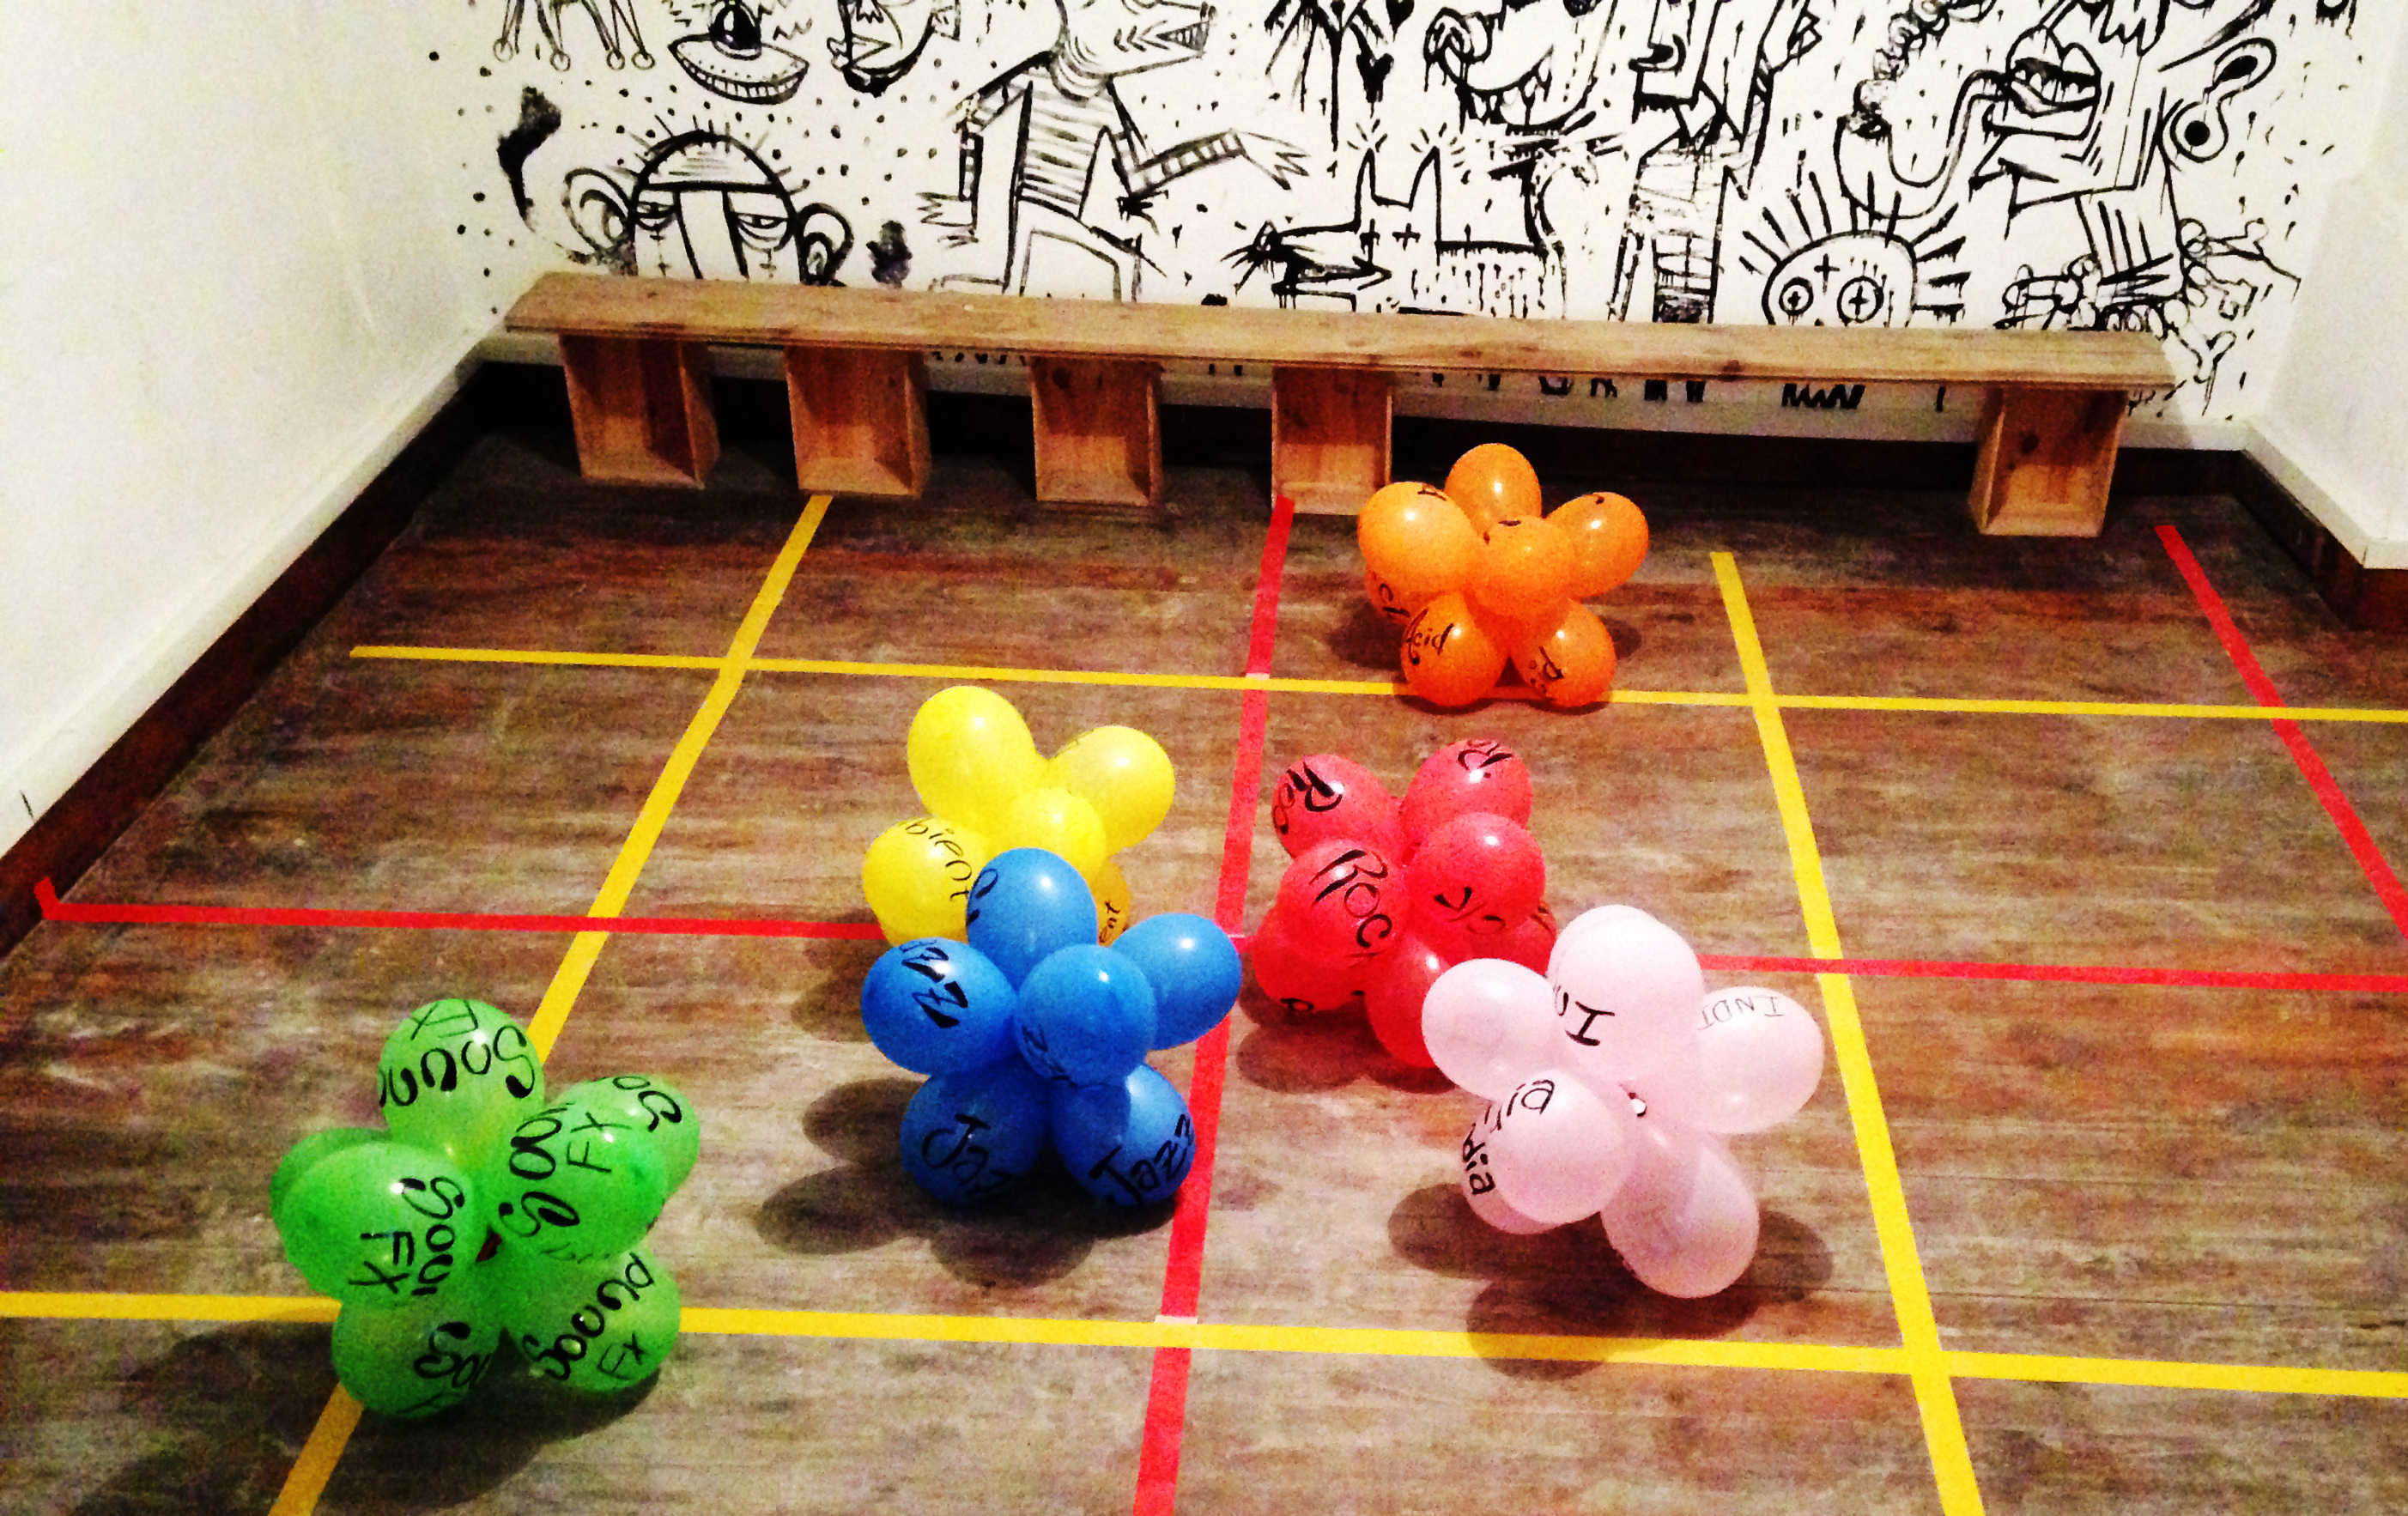
\includegraphics[width=\linewidth]{balloons}
        \caption{Balloon bundles on the dance floor (Experiment 1)}\label{fig:balloons}
\end{figure}

Figure \ref{fig:balloons} shows the system's elements on the dance floor.
It consists of a few balloon bundles, each marked with the name of a specific musical style (e.g.\ rock, jazz, Indian music).
A corresponding Bluetooth beacon is installed inside each of these bundles.
After downloading and installing the Android application, strolling between the balloon bundles affects the music in one's headphones according to the relative distance from the bundles, creating a virtual ``sound zone'' around each of them.
In addition, the distance from the center of each sound zone may affect the music in several different ways; for example, by controlling the volume, filter, and granularity of the sound zone.
Finally, participants can move the balloon bundles freely, thereby dynamically change the structure of the music in the virtual space and make it socially interactive.

Figure \ref{fig:sys:participant_view} shows an overhead view of a possible scenario of participants using the system in a party.

\begin{figure}[!htb]
	\centering
	\def\svgwidth{0.9\textwidth}
	\input{graphics/system_participant_view.pdf_tex}
	\caption{The figure depicts two participants, $A$ and $B$, dancing around three Bluetooth beacons, corresponding to the rock, jazz, and Indian music sound zones. Participant $A$ hears rock music and participant $B$ hears a mixture of the jazz and the Indian music sound zones, which are rhythmically and harmonically synchronized with each other. A video demonstration of a similar scenario can be found at \href{http://youtu.be/2kJoeD2iWBA}{youtu.be/2kJoeD2iWBA}.}\label{fig:sys:participant_view}
\end{figure}

\subsection{The BBRIP system}

The implementation of the system can be described by two different processes: the development of the BBRIP system (described in this section) and the Android application that wraps it and is responsible for the audio processing (see section \ref{sceneplayer_plus}).

The BBRIP system corresponds to my intention to develop an indoor positioning system that satisfies the relatively simple requirements of this research as presented in section \ref{methods:ips}.

My implementation of the system is based on a specific element in the Bluetooth protocol -- the Received Signal Strength Indicator (RSSI) ({\cite{bray12}).
Each Bluetooth enabled device calculates RSSI values during Bluetooth discovery, when it finds a new device and before establishing connection.

\begin{figure}[!htb]
	\centering
	\def\svgwidth{\columnwidth}
  	\input{graphics/bbrip.pdf_tex}
	\caption{The BBRIP system states and flow design}\label{fig:bbrip}
\end{figure}

As shown in Figure \ref{fig:bbrip}, the BBRIP system continuously searches for Bluetooth devices.
When a new device is found, the RSSI value is extracted and sent forward for processing.
From the first discovery in the Bluetooth discovery cycle, the system keeps checking whether the time since the last discovery exceeds a pre-defined timeout.
If so, it terminates the discovery.
This termination is important, because naturally a device can only be discovered once in each Bluetooth discovery cycle, and long periods of time without new discoveries indicates that all of the nearby devices have already been found.
Finally, when the system sees that there is no Bluetooth discovery running (because of termination or simply the end of the discovery cycle), it starts a new one immediately.

Although the RSSI values extracted by the BBRIP system are not very precise as a distance estimate, I found them sufficient to classify the distance between participants and beacons into useful ranges.
In other words, RSSI values can provide a sufficient indication of whether a participant is standing close to a specific beacon (around 1 meter), in an intermediate range (2 to 3 meters), or at a greater distance.

\subsection{ScenePlayer Plus}\label{sceneplayer_plus}

The development of the Android application transitioned through different developmental stages.

In the first phase of development the audio files that were used for playback were built into the application code-base, making the application tightly bound to a specific set of sounds and interaction opportunities.
In this early stage the application did not use ``libpd'' at all (see section \ref{methods:libpd}).
Therefore, the only effect of approaching or going away from a beacon was a change in volume.
In addition, the limited sophistication of the built-in audio library made fading in and out from the sound zones very inflexible.

After finding these weakness in the built-in audio library of the Android application programming interface, I decided to implement the system using ``libpd''.
The shift to ``libpd'' made it possible to use more advanced audio manipulations, instead of only volume changes, including, for example, filtering and granular synthesis of the audio sources.
Although the framework change presented an improvement, there was still very tight coupling between the system development in the Android environment and the audio processing development in Pd.
This tight coupling was shown by the fact that the audio sources were still embedded in the application code-base, as well as the Pd patch;
i.e., other musicians and researchers were still unable to load different musical material or different Pd patches to change the behavior of the system for their artistic or academic porpuses\footnote{First libpd based implementation source code: \href{https://github.com/Nagasaki45/ARpArty}{github.com/Nagasaki45/ARpArty}.}.

Overall, this development phase was sufficient to test the main research questions.
Nevertheless, I started to search for a better, more open architecture:
an architecture that maintains a loosely coupled connection between the Android application, the musical sources, and the Pd patch that drives the audio, and which would allow others to use the system easily.

The last phase in system development was to implement the BBRIP system into the open source Android application ``ScenePlayer''\footnote{ScenePlayer: \href{http://play.google.com/store/apps/details?id=org.puredata.android.scenes}{play.google.com/store/apps/details?id=org.puredata.android.scenes}.}, an Android port for the RjDj application mentioned in section \ref{rjdj}, and release it again as ``ScenePlayer Plus''\footnote{ScenePlayer Plus source code: \href{https://github.com/Nagasaki45/ScenePlayer-Plus}{github.com/Nagasaki45/ScenePlayer-Plus}.}.
`Scenes' in ScenePlayer are bundles of audio files and one or more Pd patches that describe, programatically, how input from the mobile device sensors should affect the audible output (\cite[p. 29]{brinkmann12}).
This design allows musicians to create Pd patches that can be uploaded to the mobile device, along with extra audio material, to create sophisticated interactions easily.
In ScenePlayer Plus, the BBRIP system is used to expose the received Bluetooth RSSI values to the Pd patch as another sensor of the mobile device (e.g.\ accelerometer, compass and touchscreen)\footnote{The scene that was used for the this research can be found at my site: \href{http://tomgurion.blogspot.com/2013/06/arparty-first-sceneplayer-plus.html}{tomgurion.blogspot.com/2013/06/arparty-first-sceneplayer-plus.html}.}.

\section{Experiment I}

To evaluate the social effects of system use I decided to conduct controlled experiments.
To Assess the system in its most natural setting the experiments were conducted in an environment resembling a silent disco party.
My purpose was to implement this specific system to explore the possibilities of using IMS in novel scenarios in the social sphere.

The main goal was to determine whether the system enhance social interaction between participants in an interactive silent disco party.
I was specifically interested to find enhanced social interactions between socially distant participants.

The social interaction between participants was assessed by self-report surveys that the participants took before, during, and after each experiment, and with objective measures such as the participants' positioning tracking and their interaction with system components.
Another goal was to evaluate the associations between the outcomes of these different methods.

The following sections present a detailed explanation of the experimental design and the results.

\subsection{Method}

\begin{figure}[!htb]
	\centering
	\def\svgwidth{0.95\columnwidth}
  	\input{graphics/pilot_design.pdf_tex}
	\caption{Experiment I design}\label{fig:pilot}
\end{figure}

Eighteen volunteers were invited to participate in an interactive silent disco party.
Each participant installed the Android application on his or her phone and filled in the pre/post party surveys that included questions regarding their musical background and preferences as well as system evaluation feedback.
The party consisted of four alternating interactive/control sessions of 5:40 minutes each (see Figure \ref{fig:pilot}).
The participants were randomly assigned to two groups: $A$ and $B$\footnote{Group $A$ (interactive first) consisted of 8 participants (4 females and 4 males) with mean age of 36.7 (s.d=12.3); group $B$ (control first) consisted of 10 participants (3 females and 7 males) with mean age of 29.6 (s.d=10.2). Participants had a diverse musical background with 4.7 mean years of musical training (s.d=5.2).}.
They were informed that the experiment consisted of interactive and control segments;
however, they were not informed about the exact schedule or timing of the sessions or the group assignments.
Both groups started the experiment together, on the same dancing floor.
In the interactive sessions, the application generated music as described in section \ref{systemdescription}, whereas in the control sessions the participants heard recorded non-interactive music created in advance using the musical material of the interactive system\footnote{The control session music composed by Noam Elron (\href{http://www.noamelron.com}{www.noamelron.com}).}.

Interaction with the system's components was assessed by counting the number of Bluetooth device discoveries made by each participant's phone during both the interactive and the control sessions.
In order to eliminate edge effects, I analyzed sensor data only from the two middle sessions of the experiment.

\subsection{Results}

\begin{figure}[!htb]
\minipage{0.49\textwidth}
	\def\svgwidth{0.95\columnwidth}
  	\input{graphics/changing_location_in_space.pdf_tex}
	\caption{Changes in locations in space}\label{fig:location}
\endminipage\hfill
\minipage{0.49\textwidth}
	\def\svgwidth{0.95\columnwidth}
	\input{graphics/dancing_with_known_people.pdf_tex}
	\caption{Dancing with known people}\label{fig:known}
\endminipage\hfill
\end{figure}

In the post-party survey, participants self-reported significantly higher levels of movement (paired t-test, $t(15)=3.9$, $p<0.01$) using the system, compared with their behavior at other parties as reported in the pre-party survey.
Figure \ref{fig:location} shows that there was a significant difference (unpaired t-test, $t(33)=6.2$, $p<0.01$) in the mean response to these questions (on a scale of 1-3).

In order to objectively assess whether participants moved more in space, I tabulated the counts of Bluetooth discoveries made by the applications' BBRIP system.
The results show slightly higher counts (paired t-test, $t(16)=1.7$, $p=0.06$, n.s) during the interactive sessions of the party than in the control sessions.
This suggests that the interactive components of the system facilitated greater participant movement in space, thereby offering more frequent opportunities for social interactions.
Indeed, in the post-party survey participants reported that they danced significantly less with people that they knew in advance, compared with their usual behavior (paired t-test, $t(14)=-2.5$, $p=0.01$).
Figure \ref{fig:known} shows that there was also a significant difference in the mean response to these questions in the pre/post surveys.
Overall, participants showed a slightly stronger tendency (paired t-test, $t(16)=1.46$ ,$p=0.08$, n.s) to participate in an interactive party in the post-party survey, compared with their response to the identical question in the pre-survey.

\subsubsection{Video analysis}\label{exp1:results:video}

\begin{figure}[!htb]
	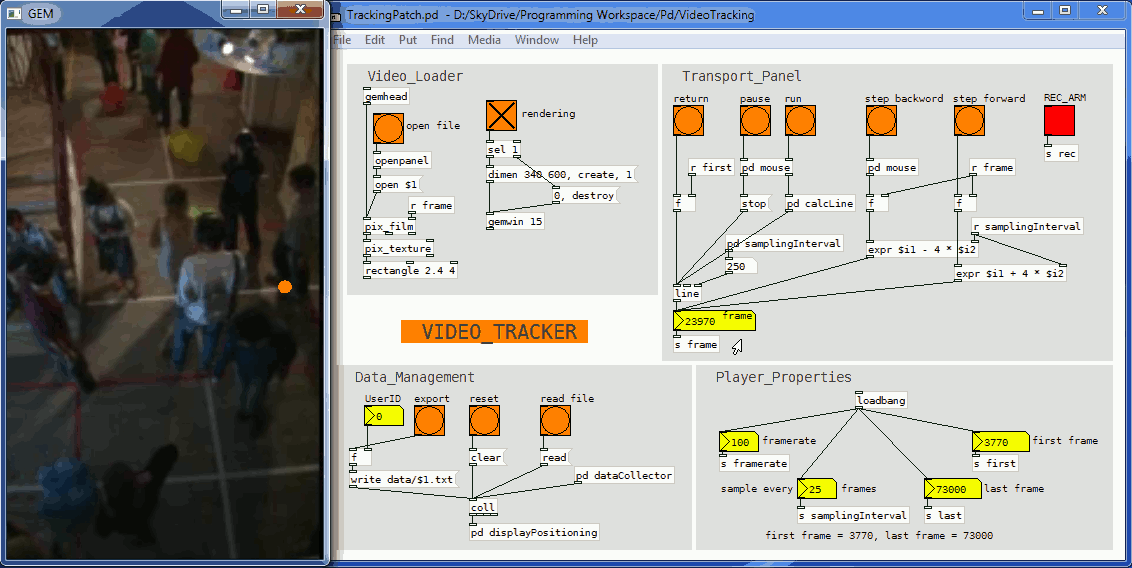
\includegraphics[width=\linewidth]{tracking}
        \caption{Pd patch for manual video tracking of participants on the dance floor}\label{fig:tracking}
\end{figure}

\begin{figure}[!htb]
    \centering
    \includegraphics[width=0.8\textwidth]{plots/pilot-familiarity_correlation_maps.pdf}
    \caption{Maps of social familiarity (on the left) and correlated movement on the dance floor (on the right)}\label{plot:pilot-familiarity_correlation_maps}
\end{figure}

The whole experiment was captured with video from a high viewing angle above the dance floor.
Later, this video was used to track the positioning of the participants and to generate positioning tables ($x$ and $y$ coordinates on the dance floor per timestamp).

Figure \ref{fig:tracking} presents the Pd patch I wrote to track the participants' movement on the dance floor using a semi-automatic procedure.
Using this patch, I tracked the positioning of each participant at a time with the computer mouse.
The location of the mouse pointer within the video window was recorded once every 25 video frames (\textasciitilde{}1 per second).
Later, I used three points on the dance floor which had been measured for their real coordinates in advance, to project the mouse tracking measurements from the video frame onto the two dimensional position of the participants on the dance floor.

No significant differences between the position and movement patterns were found between the interactive and control sessions.
However position was indicative of the social relations between participants.
I asked participants to state for their social relationships to other participants and compared the resulting map with a map of the positioning correlation between each two participants, over the entire course of the experiment\footnote{These data were measured along the Y axis alone, which was more indicative than the X axis due to the specific shape of the dance floor: The length of the dance floor (the Y axis) was 10 meters whereas the width was only 2.5 meters.}.
The obtained maps are presented in Figure \ref{plot:pilot-familiarity_correlation_maps}.
I defined the matrix similarity metric as the component-by-component squared distance and used bootstrapping resampling (\cite{good2006permutation}) to test the similarity of the maps.
As expected, I found that the matrices were significantly similar (p \textless{} 0.001).

Thus overall, these results suggest that close social relationships between participants can also be found in video analysis data.
These encouraging results prompted the design and methodology to analyze the social behavior in Experiment 2.

\subsection{Discussion}

The results support the hypothesis that system use enhances the social interaction between participants.
They suggest that audio-only augmented reality can significantly enrich the experience of music consumption and its associated social interactions.
Furthermore, they also show that the research goals can be validated in a controlled experiment using both direct reports and indirect objective measures, and that video tracking analysis can be used to identify social relationships.

However, the results do not shed light on the following points:

\begin{itemize}
	\item They do not distinguish between participants who knew one another in advance from those who did not.
	\item They do not show that the social effects of the system extend beyond the scope of this particular system use.
\end{itemize}

\section{Experiment II}

Experiment 2 was designed to clarify some of the findings from Experiment 1 and provide insights into the social effects of the system.

First, I assumed that participants at a party are pre-partitioned into groups of friends.
This assumption was based on the video analysis of Experiment 1, which showed that participants who are socially close tend to be together on the dance floor.
Therefore, there might be an association between objective measures such as video tracking results and social relations.
In addition, the same results also show well defined social clusters;
namely, that video tracking positions correspond to pre-existing social groups.
Combining the above assumption and the ability to define social clusters based on social relationships between participants I defined the \definition{in-group} and \definition{out-group} as a group of members in a social cluster a participant belongs to, and the rest of the participants respectively.
Thus Experiment 2 should shed light on the behavior of these groups as a whole and the behavior of each participant as a member of his or her own group.

Second, in Experiment 2 the control group did not experience the interactive part of the system at all.
This made it possible to compare the social behavior of the control group participants to the experiment group before and after the experiment to better understand the the long term social effects of the system.

\subsection{Method}\label{methods:evaluation}

\subsubsection{Participants}

An homogeneous class of twenty-three 11th grade pupils participated in the experiment.
The high-school was supportive and allowed me to run the experiment with the pupils using its facilities\footnote{The experiment passed the internal IRB committee of the Bar-Ilan music department. Specifically, an informed consent form was signed by the student and by the parents of each of the participants that were under 18 years old.}.

\subsubsection{Measures}

The main research question, \emph{does the system enhance social interaction between participants in an interactive silent disco party?}, was fragmented into the following operational definitions and measures\footnote{Complete version of each of the surveys can be found in the appendix.}:
\begin{enumerate}
	\item \label{measure:survey:familiarity} Participants ranked their familiarity with other participants on a scale included in the self-report questionnaire.
	\item I used the above familiarity data to cluster the participants into social groups.
  Using this clustering and the participants' positioning information (measured by video tracking as explained in section \ref{aparatus}) I defined the centroid of each cluster on the dance floor, the dispersion of the participants within each cluster and the dispersion between the cluster centroids themselves for each frame of the video.
  As presented in section \ref{results:social_structure}, I failed to find distinct social groups based on the familiarity surveys above.
  Thus in highly cohesive groups of students who knew each other in advance the video track results obtained in Experiment 1 on a non-cohesive group of subjects in which the level of familiarity varied much more could not be replicated.
  \item \label{measure:movement} Based on the assessment of movement in Experiment 1 I measured the average movement speed of the participants, hypothesizing that greater participant movement on the dance floor would provide more frequent opportunities for social interaction.
  \item \label{measure:clustering} For each frame of the video, I dynamically clustered the participants into groups based on their positioning.
  Then, I assigned scores to the clusters based on the social and positional data to obtain a better understanding of the swarming patterns of the participants.
  A detailed explanation of the techniques used for clustering can be found in section \ref{results:clustering}.
	\item \label{measure:survey:social} Participants filled out a social interaction survey.
	The survey was used to assess interaction between participants by estimating social cohesiveness within the in-group and openness to out-group interactions of each participant.
\end{enumerate}
In addition to measures intended to assess the main research question, the following operational definitions and measures were used to assess interactions and satisfaction with the system.
\begin{enumerate}[resume]
	\item \label{measure:system} I calculated the expected number of participants around a Bluetooth beacon to assess participants' interaction with the system components, where more participants around a beacon indicates greater interaction.
	\item \label{measure:survey:usability} Participants filled out a system satisfaction survey, based on the System Usability Scale (\cite{brooke96}).
\end{enumerate}
Finally, the following measures was employed to eliminate possible differences between research groups and to allow for future research based on the retrieved data.
\begin{enumerate}[resume]
	\item \label{measure:survey:musical} Participants filled out a musical background survey, based on the Emmanuel College Music Background Questionnaire, basic version (\cite{web:zhao12}).
\end{enumerate}

\subsubsection{Apparatus}\label{aparatus}

A considerable number of the measures above required participants' spatial positioning information.
To obtain this kind of positioning data I recorded the experiment with a video camera from a high viewing angle above the dance floor during the entire course of the experiment, as in Experiment 1.
Extracting the positioning of the participants was done semi-automatically, after the experiment, by tracking one participants at a time using the computer's mouse as explained in section \ref{exp1:results:video}.

The Bluetooth beacon positioning data was derived similarly, by manually tracking each of the system components in the video.

\subsubsection{Procedure}

Participants were randomly assigned to two groups, group $A$ and group $B$\@\footnote{Group $A$ consisted of 11 participants (5 females and 6 males) with a mean age of 18.7 (s.d=5.41); group $B$ consisted of 12 participants (3 females and 7 males) with a mean age of 17.2 (s.d=0.42). Participants had diverse musical backgrounds with 3.08 and 4.89 mean years of musical training (s.d=1.02 and 3.01) for groups $A$ and $B$ respectively.}.
Each group participated in the experiment on a different week, but on the same day of the week and the same hour. Group $A$ participated first and two weeks later group $B$.

\begin{figure}[!htb]
	\centering
	\def\svgwidth{0.9\textwidth}
  	\input{graphics/procedure.pdf_tex}
	\caption{Experiment design}\label{fig:experiment}
\end{figure}

First, participants filled out a musical background survey (measure \ref{measure:survey:musical}) and a participants familiarity survey (measure \ref{measure:survey:familiarity}), followed by three \definition{experimental sessions}, followed by a system usability survey (measure \ref{measure:survey:usability}).
After filling out the system usability survey the participants took part in another experimental session.
Before each experimental session and after the last one each participant filled out the social interaction survey (measure \ref{measure:survey:social}).

In each experimental session the participants listened to music on their headphones, using their Android device and pre-installed application, and interacted with other participants and system components in the `silent disco' party.
The experimental sessions were as following:

\begin{description}
	\item[Interactive:] The music generated by the Android application was identical to that described in section \ref{systemdescription}.
	\item[Control:] The music generated by the Android application was a semi-randomized sequence of the same musical material that was used in the interactive system.
  The music in the control sessions was not affected by the positioning of the participants or by the Bluetooth tokens in any way.
\end{description}

Participants in group $A$ were exposed to the following sequence of experimental sessions: Control $\rightarrow$ Control $\rightarrow$ Control $\rightarrow$ Interactive.
The participants in group $B$ were administered the sessions as follows: Control $\rightarrow$ Interactive $\rightarrow$ Control $\rightarrow$ Interactive, as shown in Figure \ref{fig:experiment}.

The procedure described above has several advantages in assessing the research questions as compared to the design in Experiment 1 and the variants of the A / B designs.
First, the interactive and control sessions effects could be compared between groups relation to the second experimental session for each group.
Second, comparisons between interactive and control sessions effects could also conducted as a within-group evaluation between the first and the second, as well as the second and third sessions of group $B$, using group $A$ as a reference.
Finally, the effects on the social interaction beyond the interactive sessions could be assessed within-group between the first and the third sessions of group $B$, using group $A$ as a reference.

Thus all the data required for analysis was collected in the first three experimental sessions.
However, the last session was added to the experiment to prevent frustration and a sense of discrimination between the groups.
Therefor, and despite the fact that the last session was not used to collect data, it was very significant in preventing group $A$ participants from biasing group $B$ results, as they were all socially close\footnote{Group $A$ participants were asked not to discuss the experiment with group $B$ participants, but since the two groups did not take the test simultaneously there was some opportunity for information to be shared across the groups. I attempted to avoid this by having an interactive session for both groups (this way the experience of both groups is similar) and by specifically asking participants to refrain from discussing their experiences.}.

\subsection{Results}

\subsubsection{System satisfaction surveys}

\begin{figure}[!htb]
    \centering
    \includegraphics[width=0.6\textwidth]{plots/usability-sus_scores.pdf}
    \caption{Mean system satisfaction scores for the control and interactive groups}\label{plot:usability-sus_scores}
\end{figure}

\begin{figure}[!htb]
    \centering
    \includegraphics[width=\textwidth]{plots/usability-per_question_statistics.pdf}
    \caption{System satisfaction questionnaire results. Bars indicates the mean response to single questions (questions are listed to the right).}\label{plot:usability-per_question_statistics}
\end{figure}

I used a system satisfaction survey at the end of the experimental sessions for each of the groups to evaluate the engagement of the participants with the system.
The survey was based on the standard system usability scale (SUS) survey (\cite{brooke96}) with minor modifications.
The SUS survey contains 10 question, 5 of which are positive (a larger number indicates greater satisfaction) and 5 of which are negative (a larger number indicates lesser satisfaction).
I used a score that combined the positive and negative questions as suggested by Brook (\cite*{brooke96}).
Figure \ref{plot:usability-sus_scores} shows that the overall system satisfaction score was higher in the interactive group (interactive: 67.3 (3); control: 45.2 (6.9); unpaired t-test, t(21) = 2.81, p \textless{} 0.01).

This effect was not limited to a single question.
In fact, four of the ten questions showed significantly higher satisfaction responses in the interactive group, as indicated by a separate one-tailed t-test (p \textless{} 0.05).
All questions except two followed the same trend (p \textless{} 0.1), and the remaining two questions (extended learning in question 10 and technician help in question 4) expected to be less relevant to this system.
These results are summarized in Figure \ref{plot:usability-per_question_statistics}.
Overall, the results consistently showed that subjects who exposed to the interactive component of the system were more satisfied than the control group who were placed in similar physical conditions.

\subsubsection{Social interaction surveys}

\begin{figure}[!htb]
    \centering
    \includegraphics[width=\textwidth]{plots/interaction_surveys-question_2.pdf}
    \caption{Mean responses to social interaction items; item 1: ``In the last experimental session I interacted with close friends only''; item 2: ``In the last experimental session I interacted with participants with whom I have no social connection''.}\label{plot:interaction_surveys-question_2}
\end{figure}

One of my main hypotheses was that the system would increase social interaction outside the native groups;
i.e., I expected that subjects who usually interact less with each other would tend to interact more.
To test this hypothesis I used a social interaction survey after each of the experimental sessions.

Surprisingly, the results of this survey showed a different trend.
The left side of Figure \ref{plot:interaction_surveys-question_2} shows the mean response (on a scale of 1 to 5) to the statement ``In the last experimental session I interacted with close friends only''.
There were no significant main effects or group by session interactions as indicated by a 2-way repeated measure ANOVA (group: F(1, 21)=0.094 p=0.762; session: F(2, 42)=0.835 p=0.441; interaction: F(2, 42)=0.548 p=0.582).

Similar results were obtained for the second question on the survey, which was ``In the last experimental session I interacted with participants with whom I have no social connection'' (group: F(1, 21)=2.062 p=0.166; session: F(2, 42)=1.730 p=0.190; interaction: F(2, 42)=1.730 p=0.190).
Note however the slight trend which indicates higher tendency to interact outside the group in the control group, as indicated by a session main effect and a significant interaction of group by session in a repeated measure 2-way ANOVA test between session one and two only (session: F(1, 21)=4.495 p=0.046; interaction: F(1, 21)=4.495 p=0.046).
Even though the overall results did not reach significance this indicates an opposite trend to the results found in Experiment 1.
In Experiment 1 subjects reported that they interacted more with subjects that they were less familiar with, though in this experiment there is no way to dissociate between using the system interactively and non-interactively.

To conclude, subjects did not appear to explicitly interact more with those outside their group;
rather, the opposite trend was observed.
As we will see this observation was further supported by the implicit measures.

\subsubsection{Social structure}\label{results:social_structure}

\begin{figure}[!htb]
    \centering
    \includegraphics[width=0.8\textwidth]{plots/familiarity-clustering_maps.pdf}
    \caption{Maps of social familiarity between participants where darker colors indicate low familiarity and lighter colors indicate high familiarity. The maps on the left are for the control group and on the right for the interactive group. From top to bottom, the maps represent the original maps, the social clustering maps using the K-means algorithm and the social clustering maps using the spectral clustering algorithm.}\label{plot:familiarity-clustering_maps}
\end{figure}

In Experiment 1, participants were recruited via the internet and therefore had varied prior familiarity with each other.
This created strong grouping into social clusters that was also apparent in their positioning in space, as indicated by my video tracking analysis in section \ref{exp1:results:video}.
Based on these encouraging results I specifically asked subjects to fill in a social familiarity survey at the beginning of the experiment.
Each participant was asked to rank his or her class peers on a scale of 1 to 5 according to social familiarity (see section \ref{methods:evaluation}).
Note that the second experiment group was much more homogeneous since unlike Experiment 1 they all came from the same high-school class.

The first row in Figure \ref{plot:familiarity-clustering_maps} shows pre-clustered social matrices, where the familiarity of each participant on the y axis with participants on the x axis is indicated by color.
I applied K-means\footnote{K-means: \href{http://scikit-learn.org/stable/modules/clustering.html\#k-means}{scikit-learn.org/stable/modules/clustering.html\#k-means}.} and spectral clustering\footnote{Spectral clustering: \href{http://scikit-learn.org/stable/modules/clustering.html\#spectral-clustering}{scikit-learn.org/stable/modules/clustering.html\#spectral-clustering}.} algorithms as implemented by the software package Scikit-learn (\cite{scikit-learn}) on these matrices but did not find a significant clustering of the participants into distinct social groups.
This is also indicated by the cross cluster similarity outside the main diagonal of the clustered matrices as depicted in the last two rows of Figure \ref{plot:familiarity-clustering_maps}.

\subsubsection{Video analysis: Movement}

\begin{figure}[!htb]
    \centering
    \includegraphics[width=0.6\textwidth]{plots/analyze-movement.pdf}
    \caption{Mean speed of participants}\label{plot:analyze-movement}
\end{figure}

Experiment 1 showed that video tracking could be used effectively to acquire insights into social interactions.
Based on these encouraging results I used extensive video tracking in Experiment 2.

I analyzed the mean speed of each participant during each session, hypothesizing that the interactive system would facilitate movement among the users.
However, I found the opposite trend, where in fact, during the second session the participants in the interactive group tended to move significantly less than those of the control group.
This trend persisted and even increased in the last session of the experiment.
This was confirmed by a significant group by session interaction in a repeated measure 2 way ANOVA test (group: F(1, 21)=3.311 p=0.083; session: F(2, 42)=0.579 p=0.455; interaction: F(2, 42)=7.318 p=0.013).
Note however, that in the first session, there was no significant difference between the groups ((interactive: 0.269 (0.048); control: 0.258 (0.035); two-tailed unpaired t-test, t(21) = -0.18, p = 0.22).

\subsubsection{Video analysis: Interaction with system components}\label{results:system}

\begin{figure}[!htb]
    \centering
    \includegraphics[width=\textwidth]{plots/annotations-clustering_example.pdf}
    \caption{Locations of participants and beacons in space for two typical point in time. Blue dots indicate the participants' locations; green indicates beacons, red indicates the bench area, yellow indicates clusters of participants and beacons.}\label{plot:annotations-clustering_example}
\end{figure}

\begin{figure}[!htb]
    \centering
    \includegraphics[width=\textwidth]{plots/annotations-correlated_movement_example.pdf}
    \caption{The correlated movement of two participants during the interactive group's second session. It is clear that these participants moved in a coordinated fashion for a time epoch of 9 seconds while holding two beacons.}\label{plot:annotations-correlated_movement_example}
\end{figure}

Figure \ref{plot:annotations-clustering_example} shows a screenshot of one point in time extracted from session 2, for each group\footnote{Animated renditions of the participants' movements can be found on my website: \href{http://tomgurion.blogspot.com/2014/10/participants-movement-tracking-videos.html}{tomgurion.blogspot.com/2014/10/participants-movement-tracking-videos.html}.}.
These animations show that participants in the interactive group tended to cluster around the interactive components of the system in small groups.

One other phenomenon found in the video animations was correlated movement of participants in the interactive group, as can be seen in the list of sequential screenshots in Figure \ref{plot:annotations-correlated_movement_example}.

\begin{figure}[!htb]
    \centering
    \includegraphics[width=0.6\textwidth]{plots/analyze-expectancy_of_participants_close_to_a_beacon.pdf}
    \caption{Expectancy for the number of participants in a 1 meter radius around a beacon}\label{plot:analyze-expectancy_of_participants_close_to_a_beacon}
\end{figure}

These anecdotal observations were confirmed by a rigorous statistical analysis.
I counted the mean number of participants near (less than 1 meter) each beacon over the frames of the video per beacon.
In each video frame, beacons that had no participants around them were excluded from the calculation.
The results are summarized in Figure \ref{plot:analyze-expectancy_of_participants_close_to_a_beacon}.
As expected from the fact that groups did not differ in the initial procedure in the first session, there was no significant difference between the groups in this session as indicated by a two-tailed unpaired t-test (interactive: 1.78 (0.071); control: 1.64 (0.20); t(10) = -0.57, p = 0.15).
However the interactive group showed a larger tendency to crowd around the beacons, as indicated by a significant group effect in a repeated measure 2 way ANOVA test (F(1, 9)=9.974 p=0.012).
This is consistent with the explicit results of the system satisfaction survey that showed that participants were more satisfied and therefore probably more engaged with the system.

\subsubsection{Video analysis: Clustering}\label{results:clustering}

\begin{figure}[!htb]
    \centering
    \includegraphics[width=\textwidth]{plots/analyze-clustering_scores.pdf}
    \caption{Clustering scores. Algorithm score is the mean distance of participants from their momentary cluster centroid. Social score is the mean of the social familiarity of the participants (as reported in the familiarity survey) with any other participant in the same cluster.}\label{plot:analyze-clustering_scores}
\end{figure}

I used the mean-shift algorithm\footnote{Mean-shift: \href{http://scikit-learn.org/stable/modules/clustering.html\#mean-shift}{scikit-learn.org/stable/modules/clustering.html\#mean-shift}.}, as implemented by the software package Scikit-learn (\cite{scikit-learn}) to cluster participants into groups based on their positioning in space.
For each frame in the video the algorithm created a number of participant clusters.
These clusters were then used to obtain the following individual participant scores:

\begin{description}
    \item[Algorithm score:] The distance of the participant from his / her cluster centroid.
        Hence lower scores indicate higher in-cluster interaction. \label{results:algorithm_score}
    \item[Social score:] The mean of the social familiarity of the participant (as reported in the familiarity survey) with any other participant in the same cluster. \label{results:social_score}
\end{description}

The final algorithm / social score for each participant is his / her average score over the frames of the whole session.

As shown in Figure \ref{plot:analyze-clustering_scores}, left plot, there was a significant difference between the second session of the interactive and the control group for the algorithm score as indicated by significant group and group by session interaction effects on a repeated measure 2 way ANOVA test (group: F(1, 21)=6.987 p=0.015; interaction: F(2, 42)=8.202 p=0.001).
Note however, that in the first session, there was no significant difference between the groups (interactive: 0.940 (0.044); control: 0.866 (0.053); two-tailed unpaired t-test, t(21) = -1.017, p=0.080).

These results indicate that when using the interactive system, participants tended to cluster in more dense clusters, confirming the observed clustering from the video animations in section \ref{results:system}.
This effect persisted over the last session, but with lesser magnitude.

Similar to the results from the interactive surveys, the right plot of Figure \ref{plot:analyze-clustering_scores} shows a non-significant group by session effect over the clusters' social scores; whereas in the interactive group participants tended to cluster with others who were socially close to them, the participants in the control group tend to cluster with participants who were distant from them socially on the social map (repeated measure 2 way ANOVA; interaction: F(2, 42)=2.032 p=0.144).

\subsection{Discussion}

Experiment 2 provides more fined grain data on the ways in which the social interactions between the participants are affected by the system.
Contrary to my expectations and the results of Experiment 1, participants self reported lower levels of interaction with people with whom they had no social connection.
This effect was supported by a non-significant measure of the social qualities of participants' ad-hoc clustering on the dance floor, showing that system usage encouraged grouping based on social familiarity.

Similarly, the participants' movement patterns showed a significant decrease in average speed as indicated by the video analysis.
This contrasted with the results of the first experiment where participants self reported higher levels of movement using the system compared to their usual behavior.

Nevertheless, the satisfaction of the participants from using the interactive components of the system was significant.
This can be seen from the system satisfaction surveys as well as from the clustering of the participants around the system components found in the video analysis.

\section{General discussion}

The experiments I conducted were designed to answer the research question: \emph{does the system enhance social interaction between participants in an interactive silent disco party?}
The two additional goals were to assess the social effects of the system beyond the scope of the experiment and the changes related to in-group cohesion as contrasted with openness to out-group interactions.

Experiment 1 targeted the main research question.
The findings confirmed the hypothesis in that the participants self reported higher levels of movement on the dance floor compared to their usual behavior, a result that was further supported by the objective measures.
Higher levels of movement can also increase the opportunities to interact with less known participants, thus suggesting a higher level of interaction with out-group participants.
The hypothesis that the system usage increases the participants' readiness to interact with the out-group was further supported by the fact that participants self reported that they danced significantly less with people they knew in advance compared to their usual behavior.

These findings prompted further use of video analysis in Experiment 2.
I decided to cluster the participants into socially homogeneous groups and use these groups in my analysis of in-group cohesiveness and openness to out-group interactions.
Unlike Experiment 1, in which participants were recruited through advertisements on the internet, the participants in the second experiment were high-school students from the same class, hence making the sample homogeneous.
This social structure impeded sufficient clustering in terms of the social relationships and therefore several analysis methods could not be used.
Thus, the terms \definition{in-group} and \definition{out-group} in Experiment 2 refer to interactions with socially close participants and less close participants respectively, since the social relationship between each dyad of participants is still a valid and useful datum.

By using video tracking I found very different movement patterns compared to Experiment 1.
Instead of higher levels of movement, as predicted, the participants in the interactive group moved much less than the control group.
This observation, combined with insights from other measures, may shed light on the social behavior of the interactive group in the experiment as will present shortly.

Despite the relatively low levels of movement in the interactive group, a qualitative observation of the movement patterns showed an interesting phenomenon: frequent occurrences of correlated movements of the participants while holding Bluetooth beacons.
This kind of correlated movement was not as common in the control group.

Another qualitative observation showed dense clusters of participants around Bluetooth beacons in the interactive group.
This observation was also backed by two independent objective measures: the expectancy of participants around a beacon and the clustering algorithm score (see sections \ref{results:system} and \ref{results:clustering} respectively).
These dense clusterings exhibited a significant difference in behavior between the interactive and the control group.

Overall, these results suggest a different model for the social effects of the system use than the one I predicted.
Instead of enhancing the interactions between participants directly, as might be concluded from the analysis of Experiment 1, participants formed dense clusters around the system's components when using the system.
Hence, the main effect is perhaps the engagement with the system and not the direct interaction between participants.
However, interaction between participants eventually occurred through joint interaction with the system's components, in an ad-hoc manner.
Furthermore, these clusters changed continuously since they were not a reflection of the social relationships between the participants or any other type of static clustering.
Thus the system created indirect opportunities for social interactions with a broad range of participants through joint engagement.

Two other results further fine-tune these insights.
First, the interaction surveys showed slight tendency in the control group to interact with less known participants compared to the interactive group, in contrast to the original hypothesis.
In addition, the clustering social score showed a similar trend, in which the participants in the control group tended to form dense clusters with less known participants compared to the interactive group.
This is consistent with the assumption that in the interactive group participants were clustered based on the beacons' positioning in an ad-hoc manner and were focused on the joint consumption of musical material.
On the other hand, in the control group, when the task became repetitive, participants were increasingly forced to create social interactions beyond the scope of their known and close friends.

Nevertheless, and similar to the results of Experiment 1, in Experiment 2 participants in the interactive group were significantly more satisfied with the system, as indicated explicitly by their self reported results in the system satisfaction survey, compared to the control group.
Additional evidence of the participants' satisfaction comes from their engagement with the system components, as measured in the expectancy of participants around a beacon (see section \ref{results:system}).
This again demonstrates that engagement measured both explicitly and implicitly was higher in the interactive group compared to the control group.

My original intention was to use the familiarity-based clustering and the interaction surveys to assess the long-terms effects of the system.
Instead, my findings are dependent on ad-hoc feature and short-term properties analyses (e.g.\ the two clustering scores and the expectancy of participants around beacons).

A comparison of the results of the two experiments suggest that the system affects different kinds of social groups differently.
A heterogeneous group, as presented in Experiment 1, showed higher levels of movement whereas the homogeneous group in Experiment 2 exhibited much lower levels of movement using the interactive system.
This may imply that the interactive components of the system facilitated interactions with broader range of participants (both known and unknown) in the heterogeneous groups, whereas the main effect of the system on homogeneous groups was the increased interaction with the system components.
The joint interaction, in this case, is a side effect of the main interaction with the system.
Further research is required to understand the difference between the experiments, but in both cases the interactive component had a \textbf{measurable} effect on the way participants interacted with the system and with each other.

Overall, and despite the differences between the experiments, there was a high correlation between the explicit and the implicit results in both experiments.
This result by itself may suggest that video tracking and other objective measures (such as the Bluetooth readings of Experiment 1) may be used in future research to assess social phenomena in similar scenarios.

In terms of the larger context of the social effects of music, as presented in section \ref{literature:social_effects}, the results are promising.
The current study tried, unintentionally at first, to do the opposite than what Brown termed as the ``nature'' of music functionality: a group behavior that increases its group's competitiveness.
I was expecting that the system would have different effects; namely, that the system would promote openness and increase the social interaction between different social groups.
In that regard, Experiment 1 showed high levels of movement and an intent to interact less with known participants and Experiment 2 showed ad-hoc clustering of participants around the system components, without striking familiarity characteristics.
Generally, this illustrates how interactive music experiences may be applied in different ways to manipulate social structures, not only toward between-group competitiveness, but also to increase openness and acceptance.

\subsection{Future research}

In this study the proposed system was evaluated within the framework of a silent disco party.
Even within this framework a number of questions regarding the long-term effect of using the system remain unanswered.
Although the goal of evaluating these long-term effects was part of the design of the second experiment, I did not obtain conclusive results.
In my opinion, a similar experimental design, but with a heterogeneous group of participants might be more appropriate as a sample to answer this question.
However, further experiments with the system were beyond the scope of the current project.

It is important to note that system use may vary beyond the silent disco setting.
As already noted, the modularity of the system architecture was a goal in itself.
This goal was not exhaustively studied in the current work, but different applications of the system should be explored in the future.
For example, an artistic study of the musical possibilities enabled by the system could be investigated, or an evaluation of system use from different perspectives.

In fact, the system has already used in another case.
Maya Magnat\footnote{\href{http://spotonisrael.com/maya-magnat-il/}{spotonisrael.com/maya-magnat-il/}.} adapted the system for an interactive installation that was presented at Tel-Aviv University.
The installation was designed to reflect her childhood memories in the university, as a daughter of a university employee.
She placed the Bluetooth tokens in various locations around an entire building, each one of which was associated with a painting, picture or short text.
Each token musical material was a short story about Magnat's childhood, told in her own voice.
The story also guides the listener where to go next.
Together, the visual elements and the audio corresponding to the token represented a part of her memories of the place.
Thus the system allowed Magnat to create an interactive location-based experience by supplying audio files and PureData patch to wrap them, with no additional programming involved.

More generally, this research may be seen as a demonstration of one of the novel possibilities new technology can make available to both artistic experiences and social behavior.
There is no doubt that these trends in interactive art and socially enhanced experiences will continue to develop rapidly and eventually merge successfully into our every-day experiences of music, art, and social media.

\begin{appendices}

\section[Musical background survey]{Musical background survey\\
	{\normalsize based on the Emmanuel College Music Background Questionnaire, basic version}}

Please first provide your basic information.

\begin{enumerate}
	\item Name: \myunderline
	\item Gender: Male / Female
	\item Age: \myunderline
	\item E-mail: \myunderline
\end{enumerate}
Please answer the following questions to the best of your knowledge.
\begin{enumerate}[resume]

	\item Please rate your overall interest in music according to the following scale

	\begin{tabular}{c c c c c}
		Not interested & & Neutral & & Very interested \\
		1 & 2 & 3 & 4 & 5 \\
	\end{tabular}

	\item Please rate your overall musical ability according to the following scale

	\begin{tabular}{c c c c c}
		Poor & & Average & & Excellent \\
		1 & 2 & 3 & 4 & 5 \\
	\end{tabular}

	\item How many hours per week do you spend listening to music?

	\myunderline

	\item What genre(s) do you listen to most? (check all that apply)

	\begin{tabular}{l l}
		{[{ \ }]} & Classical \\
		{[{ \ }]} & Country \\
		{[{ \ }]} & Jazz \\
		{[{ \ }]} & Rock \\
		{[{ \ }]} & Pop \\
		{[{ \ }]} & Non-western \\
		{[{ \ }]} & Other: (please specify) \myunderline \\
	\end{tabular}

	\item Most of the time, when you listen to music, you are

	\begin{tabular}{l l}
		( \ ) & not focused on the music, attending to a different task \\
		( \ ) & passively listening \\
		( \ ) & highly aware of musical nuances such as key changes, harmonies, etc. \\
		( \ ) & actively engaged (sing along, tap the beat, etc.) \\
	\end{tabular}

	\item About how many hours of musical activity do you engage in each week currently? (e.g.\ practice, performance)

	\myunderline

	\item \label{appendix:music:ensamble}Have you ever participated in a musical ensemble?

	\begin{tabular}{l l}
		( \ ) No \\
		( \ ) Yes, instrumental ensemble \\
		( \ ) Yes, vocal ensemble \\
		( \ ) Yes, both instrumental and vocal \\
	\end{tabular}

	\item If you answered YES to question \ref{appendix:music:ensamble}, please indicate how many years you have participated in the music ensemble

	\myunderline \ years

	\item Please list any instrument(s) that you play (including voice) and the years you play each of them, beginning with your primary instrument:

	\begin{tabular}{c c}
		Instrument &  Years playing \\
		\myunderline & \myunderline \\
		\myunderline & \myunderline \\
		\myunderline & \myunderline \\
		\myunderline & \myunderline \\
	\end{tabular}

	\item \label{appendix:music:before_break}Have you ever had any formal training in music? (If you are a self-taught musician, please also answer YES)

	\begin{tabular}{l l}
		( \ ) & YES, I had a formal training in music \\
		( \ ) & YES, I consider myself a self-taught musician \\
		( \ ) & NO \\
	\end{tabular}

\end{enumerate}
Please continue this form if you answered YES to question \ref{appendix:music:before_break}, otherwise please go directly to question \ref{appendix:music:after_break}.
\begin{enumerate}[resume]

	\item What type(s) of music training have you had? (check all that apply)

	\begin{tabular}{l l}
		{[{ \ }]} & private/small group lessons in instrument and/or voice \\
		{[{ \ }]} & institutional training \\
		{[{ \ }]} & University degree in music - list degree: \\
		{[{ \ }]} & self-taught \\
		{[{ \ }]} & other (please specify): \myunderline \\
	\end{tabular}

 	\item At what age did you begin to study music?

 	\myunderline

 	\item How long did your formal music training last?

 	\myunderline \ years
 	\item How long has it been since you last participated in formal music lessons?

	\begin{tabular}{l l}
		( \ ) & Currently have one \\
		( \ ) & Or \myunderline \ years \\
	\end{tabular}

	\item \label{appendix:music:after_break}If there is anything else that you feel is interesting or important about your musical background, please comment below:

	\rule{4.5in}{.5pt} \\
	\rule{4.5in}{.5pt} \\
	\rule{4.5in}{.5pt} \\
	\rule{4.5in}{.5pt}.

\end{enumerate}

\section{Social interaction survey}

\begin{tabularx}{\textwidth}{p{2in} | Y Y Y Y Y }
	& Strongly disagree & & & & Strongly agree \\
	\hline
	In the last experimental session I interacted with close friends only & 1 & 2 & 3 & 4 & 5 \\
	\hline
	In the last experimental session I interacted with participants with whom I have no social connection & 1 & 2 & 3 & 4 & 5 \\
\end{tabularx}

\section[System satisfaction survey]{System satisfaction survey\\
	{\normalsize based on the System Usability Scale}}

\begin{tabularx}{\textwidth}{p{2in} | Y Y Y Y Y }
	& Strongly disagree & & & & Strongly agree \\
	\hline
	I think that I would like to use this system frequently & 1 & 2 & 3 & 4 & 5 \\
	\hline
	I found the system unnecessarily complex & 1 & 2 & 3 & 4 & 5 \\
	\hline
	I thought the system was easy to use & 1 & 2 & 3 & 4 & 5 \\
	\hline
	I think that I would need the support of a technical person to be able to use this system & 1 & 2 & 3 & 4 & 5 \\
	\hline
	I found the various functions in this system were well integrated & 1 & 2 & 3 & 4 & 5 \\
	\hline
	I thought there was too much inconsistency in this system & 1 & 2 & 3 & 4 & 5 \\
	\hline
	I would imagine that most people would learn to use this system very quickly & 1 & 2 & 3 & 4 & 5 \\
	\hline
	I found the system very cumbersome to use & 1 & 2 & 3 & 4 & 5 \\
	\hline
	I felt very confident using the system & 1 & 2 & 3 & 4 & 5 \\
	\hline
	I needed to learn a lot of things before I could get going with this system & 1 & 2 & 3 & 4 & 5 \\
\end{tabularx}

\end{appendices}

\sloppy  % fixing line breaks in bibliography
\printbibliography[title={Bibliography}]
\end{document}
